%
% beispiel.tex
%
% (c) 2018 Prof Dr Andreas Müller, Hochschule Rapperswil
%
\documentclass[tikz]{standalone}
\usepackage{times}
\usepackage{amsmath}
\usepackage{txfonts}
\usepackage[utf8]{inputenc}
\usepackage{graphics}
\usetikzlibrary{arrows,intersections,math}
\usepackage{ifthen}
\begin{document}

\newboolean{showgrid}
\setboolean{showgrid}{false}
\def\breite{7}
\def\hoehe{4}

\begin{tikzpicture}[>=latex,thick]

% Povray Bild
\node at (0,0) {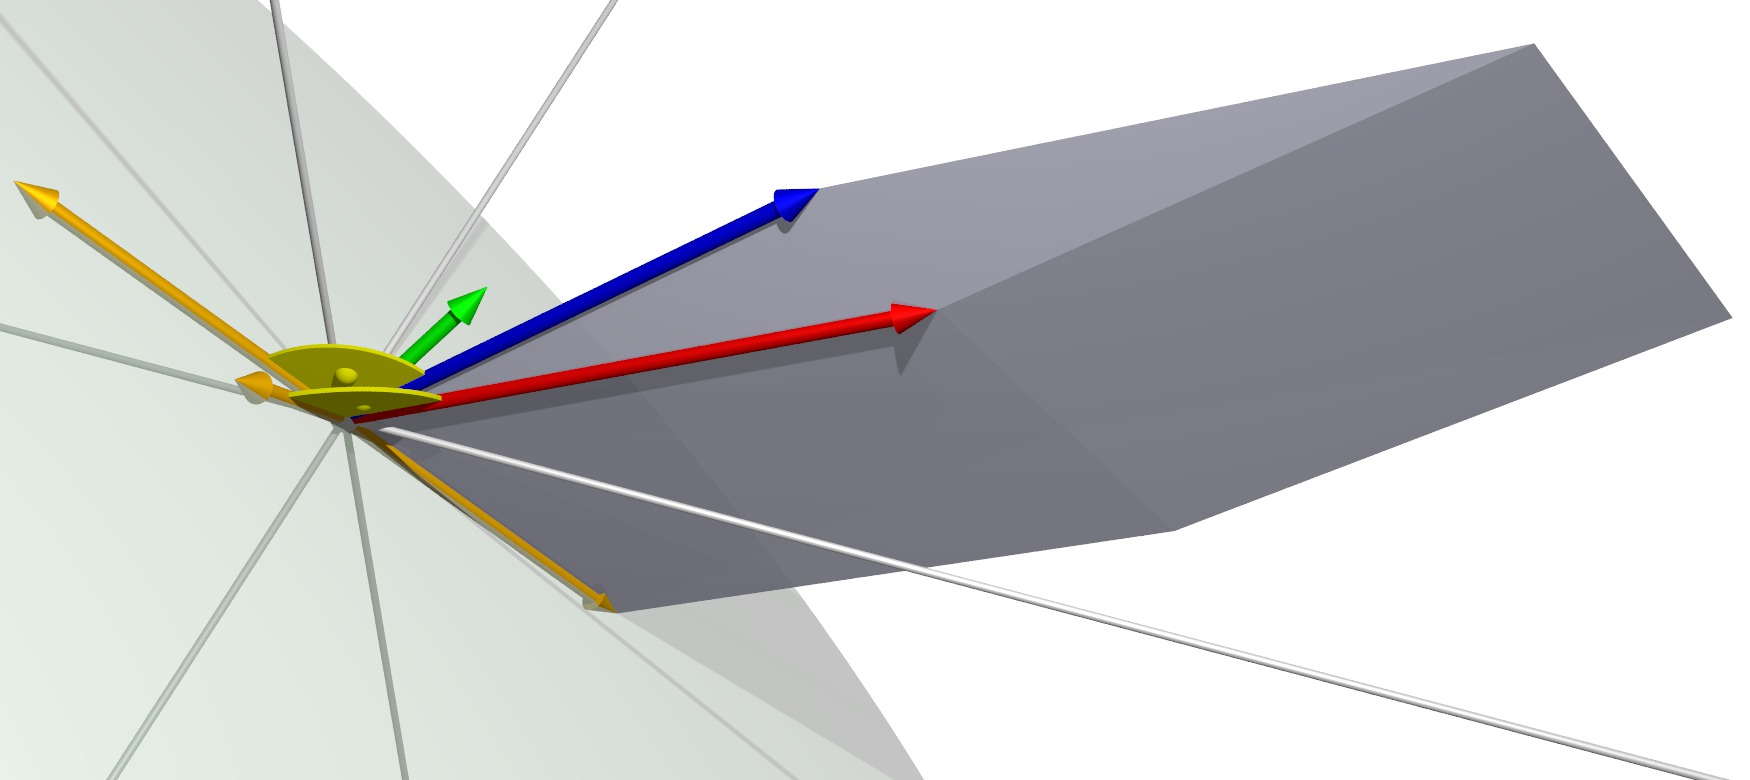
\includegraphics[width=14cm]{beispiel.jpg}};

% Gitter
\ifthenelse{\boolean{showgrid}}{
\draw[step=0.1,line width=0.1pt] (-\breite,-\hoehe) grid (\breite, \hoehe);
\draw[step=0.5,line width=0.4pt] (-\breite,-\hoehe) grid (\breite, \hoehe);
\draw                            (-\breite,-\hoehe) grid (\breite, \hoehe);
\fill (0,0) circle[radius=0.05];
}{}

\node at (-0.4,1.8) {$A$};
\node at (0.7,0.7) {$B$};
\node at (-3,1) {$\vec{n}$};

\node at (-2,-2) {$C_1$};
\node at (-6.7,1.8) {$C_2$};
\node at (-5.3,0.1) {$C_3$};

\node at (6,-2.7) {$x$};
\node at (-2,2.8) {$y$};
\node at (-4.6,2.8) {$z$};

\end{tikzpicture}

\end{document}

